%%% The main file. It contains definitions of basic parameters and includes all other parts.

%% Settings for single-side (simplex) printing
% Margins: left 40mm, right 25mm, top and bottom 25mm
% (but beware, LaTeX adds 1in implicitly)
\documentclass[12pt,a4paper]{report}
\setlength\textwidth{145mm}
\setlength\textheight{247mm}
\setlength\oddsidemargin{15mm}
\setlength\evensidemargin{15mm}
\setlength\topmargin{0mm}
\setlength\headsep{0mm}
\setlength\headheight{0mm}
% \openright makes the following text appear on a right-hand page
\let\openright=\clearpage

%% Settings for two-sided (duplex) printing
% \documentclass[12pt,a4paper,twoside,openright]{report}
% \setlength\textwidth{145mm}
% \setlength\textheight{247mm}
% \setlength\oddsidemargin{14.2mm}
% \setlength\evensidemargin{0mm}
% \setlength\topmargin{0mm}
% \setlength\headsep{0mm}
% \setlength\headheight{0mm}
% \let\openright=\cleardoublepage

%% Character encoding: usually latin2, cp1250 or utf8:
\usepackage[utf8]{inputenc}

%% Further useful packages (included in most LaTeX distributions)
\usepackage{amsmath}        % extensions for typesetting of math
\usepackage{amsfonts}       % math fonts
\usepackage{amsthm}         % theorems, definitions, etc.
\usepackage{bbding}         % various symbols (squares, asterisks, scissors, ...)
\usepackage{bm}             % boldface symbols (\bm)
\usepackage{graphicx}       % embedding of pictures
\usepackage{fancyvrb}       % improved verbatim environment
\usepackage{natbib}         % citation style AUTHOR (YEAR), or AUTHOR [NUMBER]
\usepackage[nottoc]{tocbibind} % makes sure that bibliography and the lists
			    % of figures/tables are included in the table
			    % of contents
\usepackage{dcolumn}        % improved alignment of table columns
\usepackage{booktabs}       % improved horizontal lines in tables
\usepackage{paralist}       % improved enumerate and itemize
\usepackage[usenames]{xcolor}  % typesetting in color
%\usepackage[czech]{babel}
%\usepackage[toc,page]{appendix}



\usepackage{tikz} % To generate the plot from csv
\usepackage{pgfplots}
\usepgfplotslibrary{dateplot}

%%% Basic information on the thesis

% Thesis title in English (exactly as in the formal assignment)
\def\ThesisTitle{Scalable link-time optimization}

% Author of the thesis
\def\ThesisAuthor{Ladislav Láska}

% Year when the thesis is submitted
\def\YearSubmitted{2016}

% Name of the department or institute, where the work was officially assigned
% (according to the Organizational Structure of MFF UK in English,
% or a full name of a department outside MFF)
\def\Department{ Computer Science Institute of Charles University }


% Is it a department (katedra), or an institute (ústav)?
\def\DeptType{Institute}

% Thesis supervisor: name, surname and titles
\def\Supervisor{Mgr. Jan Hubička Ph.D.}

% Supervisor's department (again according to Organizational structure of MFF)
\def\SupervisorsDepartment{Computer Science Institute of Charles University}

% Study programme and specialization
\def\StudyProgramme{Informatics}
\def\StudyBranch{Discrete Models and Algorithms}

% An optional dedication: you can thank whomever you wish (your supervisor,
% consultant, a person who lent the software, etc.)
\def\Dedication{%
Dedication.
}

% Abstract (recommended length around 80-200 words; this is not a copy of your thesis assignment!)
\def\Abstract{%
\TODO{This is assignment. Replace with proper abstract!}
Moderní překladače programovacích jazyků obsahují velké množství optimalizací,
které vedou ke zrychlení a zmenšení výsledného programu. V posledních letech
je stále častějších optimalizovat program jako celek místo tradičního modelu,kde
se jednotlivé zdrojové soubory přeloží a optimalizují samostatně. Tento postup
vede k nutnosti řešit probémy nad velkými grafy, které často obsahují desítky až
miliony vrcholů. Optimalizace navržené pro výrazně menší jednotky překladu pak
vyžadují nepřiměřené množství času a paměti.

Řešitel prostuduje datové strukty určené k práci nad velkými grafy a seznámí se
s implementací jednotlivých optimalizací v GNU Compiler Collection (GCC) se
zaměřením na interprocedurální points-to analýzu. Posoudí praktickou
použitelnost pokročilých datových struktur a algoritmů ke zlepšení
škálovatelnosti a prakticky implementuje vybrané z nich.
}

% 3 to 5 keywords (recommended), each enclosed in curly braces
\def\Keywords{%
{key} {words}
}

%% The hyperref package for clickable links in PDF and also for storing
%% metadata to PDF (including the table of contents).
\usepackage[pdftex,unicode]{hyperref}   % Must follow all other packages
\hypersetup{breaklinks=true}
\hypersetup{pdftitle={\ThesisTitle}}
\hypersetup{pdfauthor={\ThesisAuthor}}
\hypersetup{pdfkeywords=\Keywords}
\hypersetup{urlcolor=blue}

% Definitions of macros (see description inside)
%%% This file contains definitions of various useful macros and environments %%%
%%% Please add more macros here instead of cluttering other files with them. %%%

%%% Minor tweaks of style

% These macros employ a little dirty trick to convince LaTeX to typeset
% chapter headings sanely, without lots of empty space above them.
% Feel free to ignore.
\makeatletter
\def\@makechapterhead#1{
  {\parindent \z@ \raggedright \normalfont
   \Huge\bfseries \thechapter. #1
   \par\nobreak
   \vskip 20\p@
}}
\def\@makeschapterhead#1{
  {\parindent \z@ \raggedright \normalfont
   \Huge\bfseries #1
   \par\nobreak
   \vskip 20\p@
}}
\makeatother

% This macro defines a chapter, which is not numbered, but is included
% in the table of contents.
\def\chapwithtoc#1{
\chapter*{#1}
\addcontentsline{toc}{chapter}{#1}
}

% Draw black "slugs" whenever a line overflows, so that we can spot it easily.
\overfullrule=1mm

%%% Macros for definitions, theorems, claims, examples, ... (requires amsthm package)

\theoremstyle{plain}
\newtheorem{thm}{Theorem}
\newtheorem{lemma}[thm]{Lemma}
\newtheorem{claim}[thm]{Claim}

\theoremstyle{plain}
\newtheorem{defn}{Definition}

\theoremstyle{remark}
\newtheorem*{cor}{Corollary}
\newtheorem*{rem}{Remark}
\newtheorem*{example}{Example}

%%% An environment for proofs

%%% FIXME %%% \newenvironment{proof}{
%%% FIXME %%%   \par\medskip\noindent
%%% FIXME %%%   \textit{Proof}.
%%% FIXME %%% }{
%%% FIXME %%% \newline
%%% FIXME %%% \rightline{$\square$}  % or \SquareCastShadowBottomRight from bbding package
%%% FIXME %%% }

%%% An environment for typesetting of program code and input/output
%%% of programs. (Requires the fancyvrb package -- fancy verbatim.)

\DefineVerbatimEnvironment{code}{Verbatim}{fontsize=\small, frame=single}

%%% The field of all real and natural numbers
\newcommand{\R}{\mathbb{R}}
\newcommand{\N}{\mathbb{N}}

%%% Useful operators for statistics and probability
\DeclareMathOperator{\pr}{\textsf{P}}
\DeclareMathOperator{\E}{\textsf{E}\,}
\DeclareMathOperator{\var}{\textrm{var}}
\DeclareMathOperator{\sd}{\textrm{sd}}

%%% Transposition of a vector/matrix
\newcommand{\T}[1]{#1^\top}

%%% Various math goodies
\newcommand{\goto}{\rightarrow}
\newcommand{\gotop}{\stackrel{P}{\longrightarrow}}
\newcommand{\maon}[1]{o(n^{#1})}
\newcommand{\abs}[1]{\left|{#1}\right|}
\newcommand{\dint}{\int_0^\tau\!\!\int_0^\tau}
\newcommand{\isqr}[1]{\frac{1}{\sqrt{#1}}}

%%% Various table goodies
\newcommand{\pulrad}[1]{\raisebox{1.5ex}[0pt]{#1}}
\newcommand{\mc}[1]{\multicolumn{1}{c}{#1}}

\newcommand{\TODO}[1]{{\bf\Large TODO: #1}}

\usepackage{kmath}

% Title page and various mandatory informational pages
\begin{document}
%%% Title page of the thesis and other mandatory pages

%%% Title page of the thesis

\pagestyle{empty}
\hypersetup{pageanchor=false}
\begin{center}

\centerline{\mbox{
\includegraphics[width=166mm]{img/logo-en.pdf}}}

\vspace{-8mm}
\vfill

{\bf\Large MASTER THESIS}

\vfill

{\LARGE\ThesisAuthor}

\vspace{15mm}

{\LARGE\bfseries\ThesisTitle}

\vfill

\Department

\vfill

\begin{tabular}{rl}

Supervisor of the master thesis: & \Supervisor \\
\noalign{\vspace{2mm}}
Study programme: & \StudyProgramme \\
\noalign{\vspace{2mm}}
Study branch: & \StudyBranch \\
\end{tabular}

\vfill

% Zde doplňte rok
Prague \YearSubmitted

\end{center}

\newpage

%%% Here should be a bound sheet included -- a signed copy of the "master
%%% thesis assignment". This assignment is NOT a part of the electronic
%%% version of the thesis. DO NOT SCAN.

%%% A page with a solemn declaration to the master thesis

\openright
\hypersetup{pageanchor=true}
\pagestyle{plain}
\pagenumbering{roman}
\vglue 0pt plus 1fill

\noindent
I declare that I carried out this master thesis independently, and only with the cited
sources, literature and other professional sources.

\medskip\noindent
I understand that my work relates to the rights and obligations under the Act No.~121/2000 Sb.,
the Copyright Act, as amended, in particular the fact that the Charles
University has the right to conclude a license agreement on the use of this
work as a school work pursuant to Section 60 subsection 1 of the Copyright Act.

\vspace{10mm}

\hbox{\hbox to 0.5\hsize{%
In Prague date January 1st 2017	% FIXME!
\hss}\hbox to 0.5\hsize{%
signature of the author
\hss}}

\vspace{20mm}
\newpage

%%% Mandatory information page of the thesis

\openright

\vbox to 0.5\vsize{
\setlength\parindent{0mm}
\setlength\parskip{5mm}

Title:
\ThesisTitle

Author:
\ThesisAuthor

\DeptType:
\Department

Supervisor:
\Supervisor, \SupervisorsDepartment

Abstract:
\Abstract

Keywords:
\Keywords

\vss}

\newpage

%%% Dedication

\openright

\noindent
\Dedication

\newpage

\openright
\pagestyle{plain}
\pagenumbering{arabic}
\setcounter{page}{1}


%%% A page with automatically generated table of contents of the master thesis

\tableofcontents

%%% Each chapter is kept in a separate file
\chapter*{Preface}
\addcontentsline{toc}{chapter}{Úvod}

%Dosavadní implementace alias analýzy v GCC je založena na článcích [Efficient
%Field-sensitive pointer analysis for C" a "Ultra-fast Aliasing Analysis using
%CLA: A Million Lines of C Code in a Second".
%
%Pro výpočet analýzy používá constraint-graph, který obsahuje výrazy typu
%Dereference, vzetí adresy, a skalární, nad kterými spočítá (?) tranzitivní
%uzávěr a vydedukuje points-to množiny. 
%
%Toto má mnohé nevýhody, zejména praktickou nepoužitelnost při optimalizacích
%celých programů (? IPA a LTO).
%
%Právě na téma škálovatelnosti se v posledních letech upřely zraky mnohých 
%akademiků i programátorů. Příchod LTO a existence programů obrovských rozměrů, 
%jako je například Firefox či KDE, zapříčinily, že standardní postupy již nejsou 
%použitelné.
%
%Cílem této práce je navrhnout algoritmy a datové struktury, které budou
%dostatečně rychlé a prostorově úsporné, aby byly použitelné při kompilaci
%velkých programů bez potřeby superpočítačů.

As soon as programs started their growth, it became necessity to split them into
functions, and later into compilation units. This shields the programmer from
unnecessary technical details of implementation, and allows him to concentrate on
the actual work.

Unfortunately, this is also true for the compiler, which is shielded from the
implementation details. However in this case, the implementation details are not
unnecessary and the compiler could do a better job if it knew.

For a long time, most compilers worked on separate compilation units, and didn't
really care about other units in terms of analysis.

In the recent years, computing power of consumer-grade machines increased to the
point where something could be done about it, even for some bigger programs.

In 2009 the GCC merged LTO into version 4.5, which enables optimizations on the
scope of all compilation units.

The goal is to explore current link-time optimization techniques, identify a
bottleneck, and improve upon it.




I will introduce link-time optimization techniques in the first chapter,
introduce Alias Analysis problem and it's possible solutions in the second
chapter, with emphasis on practical use in current compilers. I will improve
upon Andersen's inclusion-based algorithm in the third chapter, by using
efficient data-structure derived from Bloom filters, sacrificing some precision
for tractability, and compare the results with non-approximate solution using
the same algorithm. In the last chapter, I will compare my implementation with
already available implementations in production compilers with respect to
resource use during compilation and their usability for large programs.


%Klasický přístup k překládání programů je založen na separaci kódu tak, že
%jednotlivé překladové jednotky (typicky složené z několika málo souborů) se
%přeloží najednou, a až po přeložení všech jednotek se program slinkuje do
%jednoho výsledného objektu.
%
%Tento přístup šetří zdroje počítače, který překlad provádí: jednak není nikdy
%zapotřebí mít nahraný celý program v paměti, dále je možno paralelizovat a
%překládat jednotlivé jednotky nezávisle. Nadruhou stranu však tento přístup
%zbraňuje překladači provádět optimalizace na rozhraní překladových jednotek.
%
%S tím, jak roste síla počítačů, a zejména dostupné paměti, je možné kompilační
%jednotky dále zvětšovat a pokoušet se o optimalizaci programů jako celku.
%
%Některé projekty se daly vlastní cestou, a tento problém vyřešili
%předzpracováním, které celý zdrojový kód vložilo do jednoho souboru; příklad
%může být SQLite, oblíbená relační SQL databáze, v jednom souboru obsahujícím cca
%370 řádek kódu v jazyce C.
%
%U větších projektů, jako například KDE, známé desktopové prostředí, se však brzy
%stane tento postup neunesitelný, a to zejména díky zdrojům, které jsou zapotřebí
%na překlad programu, a také díky nemožnosti snadno paralelizovat, což v dnešní
%době vícejádrových procesorů je nedostatek zcela zásadní.
%
%Tato bariéra je částečně odstraněna zavedení možnosti vložit do částečně
%přeloženého objektu dostatek metadat na to, aby ve fázi linkování šlo spustit
%některé optimalizační průchody, tzv. LTO (Link Time Optimization).
%
%Některé optimalizační průchody však byly navrženy dosti neefektivně s tím, že
%fungují dobře na jednotlivých funkcích, uspokojivě na menších překladových
%jednotkách, ale již dobře neškálují na celé programy, a to jak potřebným
%výpočetním časem, tak prostorem, a to i o několik řádů.
%
%Cílem této práce je zanalyzovat stav optimalizací, které aktuálně nejsou
%použitelné, navrhnout a implementovat řešení.
%

\newcommand{\definice}{\paragraph{Definice.}}

\chapter{Compilation and optimization}

In this chapter, we will discuss the composition of modern
programs, organization and size of their code-base. We will continue with an
overview of compilation stages, introduce optimization passses and link-time
optimization framework.

\section{Code-base organization and size}

Let us start by examining some of the code-bases for programs we use every day.
Many developers run Linux, Firefox (or other browser) and GCC, but
unless they are developing one of them, they do not really have a good idea of how large
they are. The chart in Figure \ref{figure-loc} show historical development of
code-base size over the past 10 years for selected projects.

\begin{figure}[h!]
\label{figure-loc}
\centering
	\hspace{-1cm}\includegraphics{graphs/loc/loc.pdf}
\caption{Codebase size of Firefox, Chrome and GCC over time. \TODO{citace
	openhub.net}}
\end{figure}

It might be tempting to say that the code will be split into many libraries. It
is no secret that, for example, Firefox bundles many libraries inside. They
could be compiled into separate dynamic libraries, and linked at runtime. Figure
\ref{figure-firefox-objsize} shows 8 largest libraries contained in a standard
Firefox distribution. The size of main library is 66.39 MB, while the second
largest is only 1.51 MB. This is due to speed optimizations, as the developers
noticed a significant start-up delay if all libraries are loaded separately, and
bundled them together into a single library. This also means that compiler
optimizing this library has to deal with all the code at included.

\begin{figure}[h!]
\label{figure-firefox-objsize}
\centering
\includegraphics[angle=-90,trim=0 30 10 0,clip]{graphs/firefox-objsize/objsize.pdf}
\caption{Firefox 50.0.2 object sizes by binary}
\end{figure}

We should keep these numbers in mind while designing a compiler. Compiler has
to keep up with the enormous code-base growth of projects, adding around 2
millions of lines of code each year.

\section{Program compilation}

Only the simplest programs consist of a single source file. Many programs have
tens, hundreds or even thousands of source files. This not only serves an
organizational purpose, but also allows the programmer to choose different
optimization flags for different files, or even write different parts in
different languages. A mechanism called {\sl separate compilation} is used to
compile and combine (link) all of them together, to form a finished program.
Figure \ref{figure-non-lto-workflow} shows the transformation using standard GCC
and Binutils (compiler and linker).

In this traditional model, first step is to compile every  source file into
object file. In this phase, a compiler is invoked and does all the work
necessary to convert source code into binary, including code generation. The
result is stored in an object file, including required metadata, for example,
symbol table. This step is independent for each source file, so they can be
processed in parallel. 

Second step consists of linking. The linker inspects all generated objects,
resolves required and provided symbols, dynamic libraris, and produces a
final executable. The linker usually does not modify code in object files, as it
only understands symbols and sections.

\begin{figure}[h!]
\label{figure-non-lto-workflow}
\centering
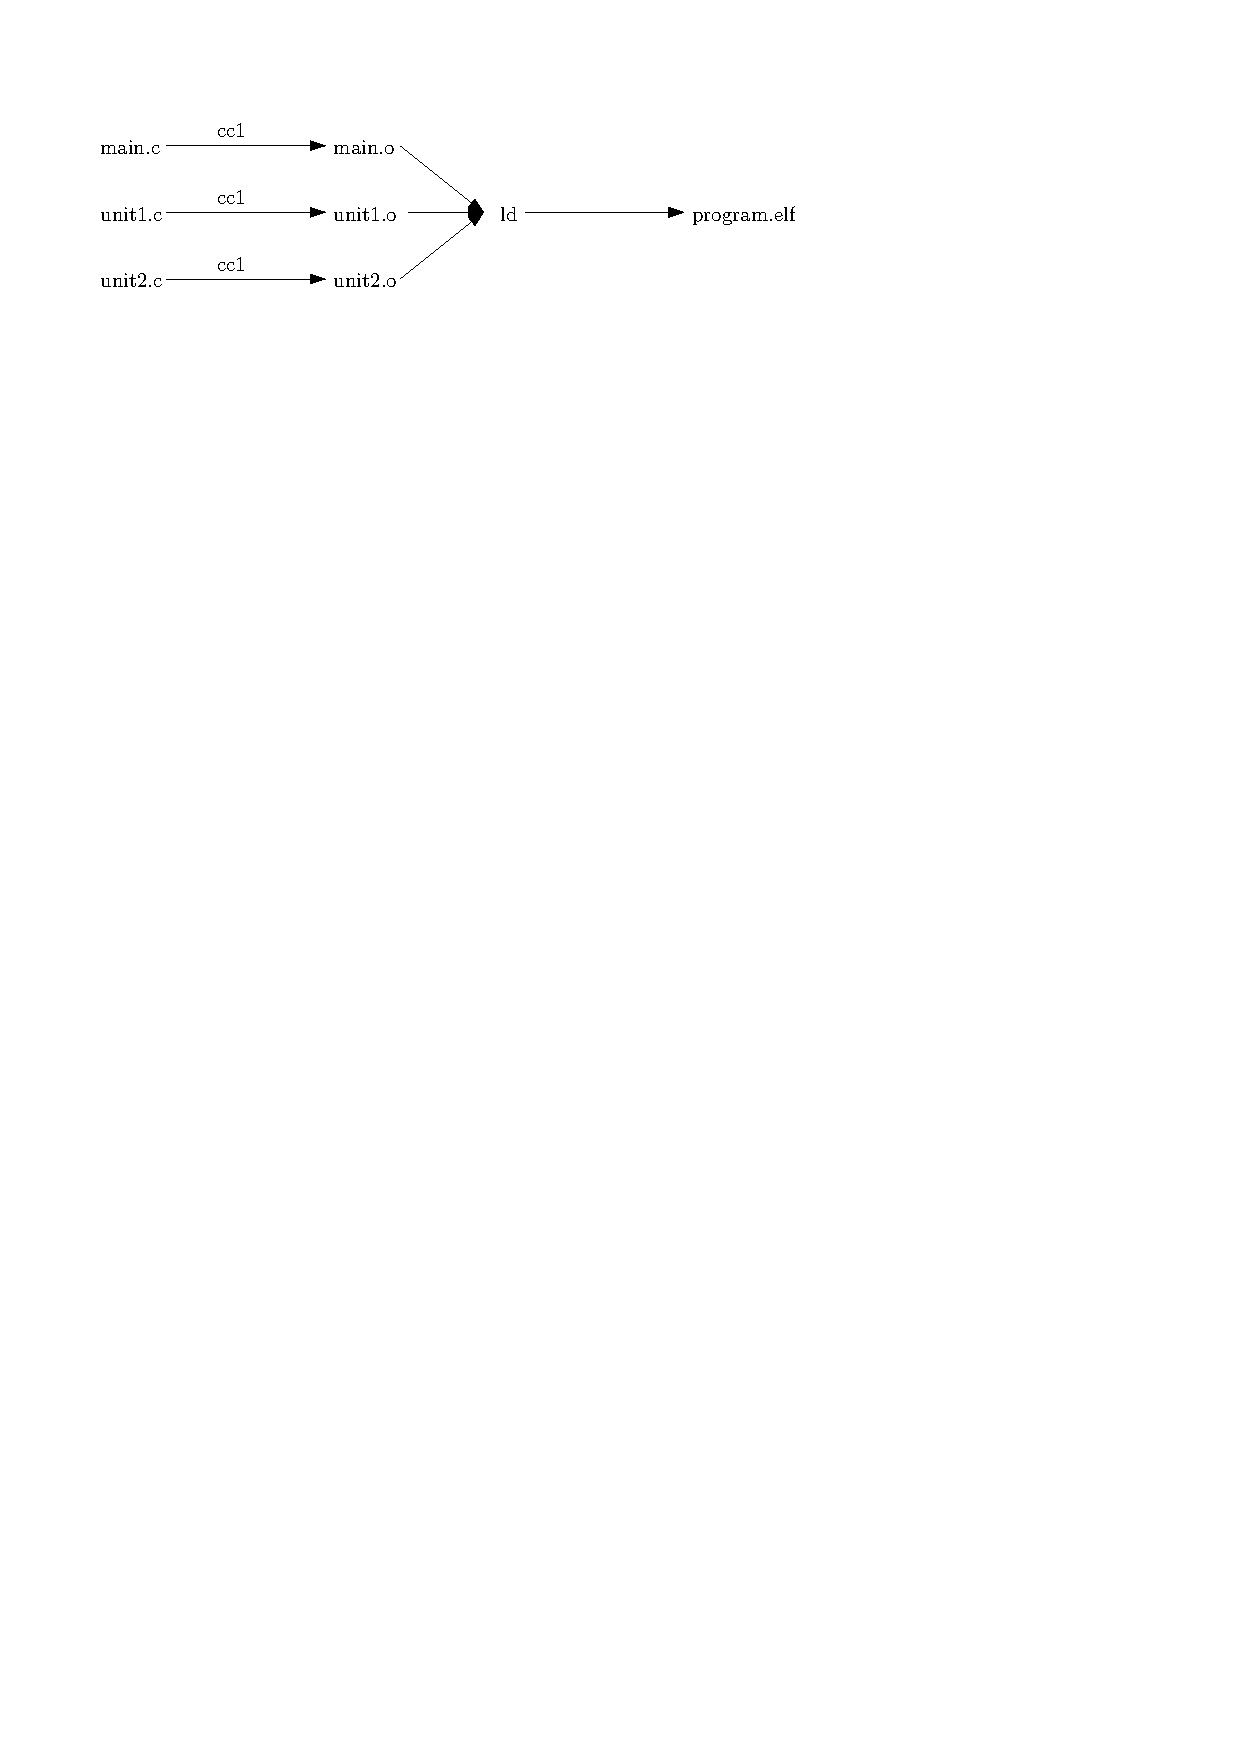
\includegraphics{./img/non-lto-workflow.pdf}
\caption{Standard workflow for separate compilation}
\end{figure}


\section{Compilation phases}

To compile a program written in a high-level programming language into a machine
code requires many steps. To make orientation easy, and to support code
re-usability, a compiler usually consists of the following parts:

\paragraph{Front End} parses the input language, builts abstract syntax
tree and converts it into a common intermediate language (IL) to all front ends
and the middle end.

\paragraph{Middle End} analyses the program represented in IL and performs most
highlevel optimizations. This includes splitting the code into basic blocks,
building a callgraph and control flow graph. Various optimizations are then
performed.

\paragraph{Back End} converts IL code into machine code, optimizing on the
lowest level, being able to schedule individual instructions and registers.

During this process multiple intermediary languages are used, sometimes more at
the same time (usually during transition to the lower-level language).

\begin{description}
	\item[GENERIC] is the highest-level IL used by the Front End, able to
		represent syntax trees and language-specific features.
	\item[GIMPLE] is tuple-based IL language, able to represent only simple
		expressions common to all languages. It is unable to represent many
		high-level constructs, for example, loops.
	\item[RTL] (Register Transfer Language) is a low level language similar to
		machine code, containing algebraicly described instructions, as should
		be generated.
\end{description}


\section{Link-time optimization}

The scope limitation imposed by separate compilation is a major block for many
optimizations. One example is devirtualization in C++. As the class it's
descendants are usually in a separate file, the compiler has no way of knowing
that there is only one possible virtual method, and devirtualize it.  This often
happens when using Mock objects\footnote{Objects that mimic some behavior, for
example a piece of hardware} for testing.

The idea of interprocedural and link-time optimization (LTO) is old. 
It was already discusses in literature in 1970s \cite{Allen:1974,Allen:1976}.
One of the first industrial strength implementation of LTO optimizing compiler
was MIPSPro, which was later released in 2000 as Open64 under GNU GPL. The
compiler suite LLVM supports link-time optimization by design, from their first
release in 2002 \cite{lattner2002llvm}.  GCC was late with their link-time
optimization framework was proposed in 2005 \cite{gcclto,briggs2007whopr} and
released in 2009.

Some developers worked around this limitation. For example, SQLite or older versions
of KDE support code concatenation in their build system. This results in one
huge source file being passed to the compiler. The result was good in its day,
but still had some issues. All the code needs to be parsed at once, which
increases memory usage and does not scale well, as language parsers are not
usually parallel, and thus cannot make use of multi processor system.

\begin{figure}[h!]
	\label{figure-lto-workflow}
	\centering
	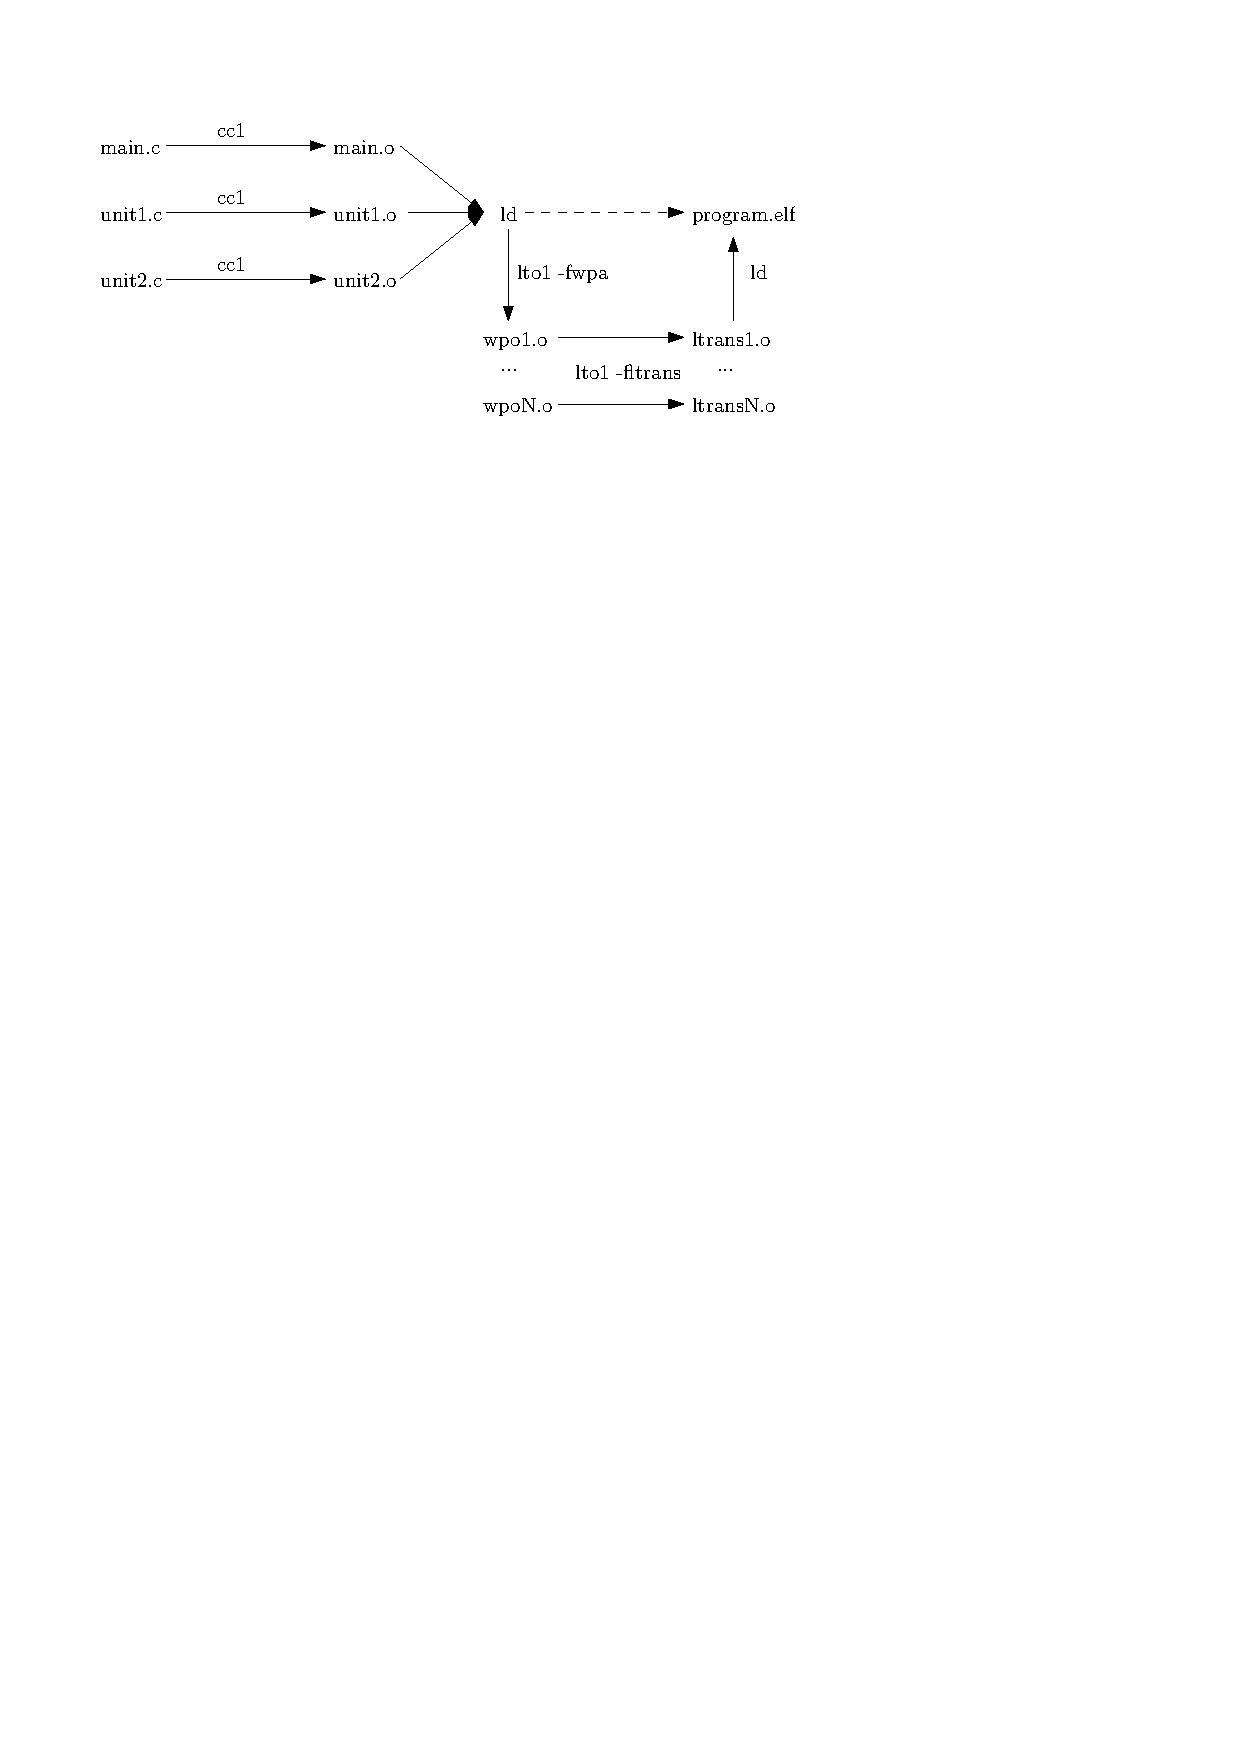
\includegraphics{./img/lto-workflow.pdf}
	\caption{Compiling source code into binary}
\end{figure}

The LTO framework (see Figure \ref{figure-lto-workflow}) solves these problems by keeping separate compilation, but
instead of generating classical object files containing machine code, the
middle end stops and writes GIMPLE representation into the object, including
some metadata (for example the call graph).

Instead of generating library, the linker then picks up the GIMPLE
representation and invokes the compiler again. GCC was designed to perform most
of the optimizations in parallel, and the process has been further split into
two stages. The sequential WPA (Whole Program Analysis) stage and parallel
LTRANS (Local TRANSformations) stage.

\paragraph{WPA} stage performs declaration and type linking, and decision stage
of interprodecural optimizations. It ends by partitioning the code into smaller
pieces called {\sl LTO partitions}. The partitioning happens with regard to the
code being optimized, for example to minimize cross-partition edges.

\paragraph{LTRANS} stage then performs optimizations decided by WPA stage,
followed by local optimizations and code generation.


\section{Evaluating GCC performance}

As we previously noted, we will be focusing on the GCC compiler suite. In this
section, we will cover the experimental setup, evaluate compile time in selected
programs and extract practical information on resources needed and anticipated
use.  The source code used to take these measurements is available online (See
\TODO{ref}, allowing others to reproduce results presented and use it in future
work.  

\subsection{Compiler}

For further measurements, we will the 5.3 release of GCC. This release is
relatively fresh, supports most of the latest features, but will not change
during the development. It will provide stable base for testing, while still
receiving bug fixes for the time being. 

\subsection{Software under test}

Several opensource programs are available for testing, however a good candidate has
to be selected in order to make testing straightforward and reproducible.
We will choose testing applications based on the following criteria:

\begin{itemize}
	\item written in C++ (preferred) or C,
	\item good compatibility with current GCC versions (5.x and 6.x),
	\item flexible and robust build system,
	\item mid to large codebase,
	\item and preferably large monolithic binary.
\end{itemize}

It is surprisingly difficult to find projects that fit all of those
requirements. For example the build systems of MySQL and Inkscape is very
inflexible and has trouble with LTO compilation. GIMP consists of many plugins
which does not pose any challenge for the current link-time optimizer. The
following applications were used in this work.

\paragraph{Firefox} is already an established benchmark for GCC \cite{glek2010}
and though earlier versiond were difficult to build with LTO, recent versions
are polished and fullfill all the requirements. Is is the largest test case and
though it takes only a few minutes to compile in standard setup, the time can be
raised to many hours with certain optimizations enabled. We will discuss this in
more detail later in Section \ref{section-firefox-lto-pta}. Besides the size,
the codebase is also divers and makes use of modern C++ constructs. The specific
version used in testing is {\it Firefox 48}.

\paragraph{Merkaartor} is an OpenStreetMap editor written in C++ with medium
sized code-base. It utilizes Qt framework, a lot of C++ constructs and links
plenty of objects into a single binary, and uses a lot of C++ constructs.  The
specific version used in testing is {\it Merkaartor 0.18.3-rc1}

\paragraph{SQLite} is a SQL database engine in a single source file with a
medium (to small) sized code-base. It is the simplest of all three and does not
offer much challenge for the optimizer, but offers very quick turn time as well
as an easy entry point for testcase minimization. The specific version used in
testing is {\it SQLite 3.8.7.4}.

\subsection{Experimental setup}

Where relevant, the following machine was used for testing:

\begin{itemize}
	\item Intel Xeon E3-1231-v3 @ 3.40GHz (Haswell)
	\item 32GB DDR3 RAM @ 1600MHz, 4 modules KHX1600C10D3/8G
	\item 120GB Intel 520 SSD, SSDSC2CW120A3
\end{itemize}

This setup is on the high-end of desktop computing, and much more than
should be required for regular development. 

The system was running 64bit Linux kernel 4.5 and standard Gentoo Linux
installation. Memory and CPU usage measurements were taken using Linux Control
Groups \TODO{cite} for whole compilation process, including GNU make and other tools. The
data were sampled at 1 second intervals, which is more than enough. Total CPU
usage is known precisely, as control groups keep cumulative counter. The
activity at a given point is used only as a pointer as to how many cores are
currently computing. As for the memory, the second interval is fine as well, as
we are not allocating and freeing memory rapidly. In fact, most of our
allocations will be done at the beginning of an analysis.

\subsection{Compiling Firefox with LTO and IPA PTA}
\label{section-firefox-lto-pta}

Firefox, in a standard configuration, can be compiled within minutes. See Figure
\ref{figure-firefox-nolto} for a graph of the whole compilation (not only the
{\tt libxul.so}). The dip in CPU cores used around 16th minute is the linker for
{\tt libxul.so} being invoked, the following spike is a parallel compilation of a few
unit tests and miscellaneous parts.

\begin{figure}[h!]
	\label{figure-firefox-nolto}
	\centering
	\includegraphics{./graphs/firefox-nolto/firefox-ipa-pta.pdf}
	\caption{Compiling firefox without LTO}
\end{figure}

Enabling LTO results in slightly longer compile time, but most of the time is
spent during the LTO phase of {\tt libxul.so}, which is plotted separately in Figure
\ref{figure-firefox-lto8}.

Enabling the interprocedural alias analysis pass causes the compilation to end
abruptly due to insufficient RAM.  See Figure \ref{figure-firefox-ipa-pta-lto8}
for details: each drop in utilized CPU cores shows a moment where one LTO
process was killed by the kernel on OOM condition (or finished successfully in
later phases). This issue is remedied by running only 2 processes concurrently
(see Figure \ref{figure-firefox-ipa-pta-lto2}).  However even in this setup the
compiler used more than 27 GB RAM and it took around 18 hours to complete.

\begin{figure}
\begin{subfigure}[b]{\textwidth}
	\label{figure-firefox-lto8}
	\centering
	\includegraphics{./graphs/firefox-lto8/firefox-ipa-pta.pdf}
	\caption{{\tt libxul.so} with {\tt -flto=8}}
\end{subfigure}
\begin{subfigure}[b]{\textwidth}
	\label{figure-firefox-ipa-pta-lto8}
	\centering
	\includegraphics{./graphs/firefox-ipa-pta-lto8/firefox-ipa-pta.pdf}
	\caption{{\tt libxul.so} with {\tt -fipa-pta -flto=8}}
\end{subfigure}
\begin{subfigure}[b]{\textwidth}
	\label{figure-firefox-ipa-pta-lto2}
	\centering
	\includegraphics{./graphs/firefox-ipa-pta-lto2/firefox-ipa-pta.pdf}
	\caption{{\tt libxul.so} with {\tt -fipa-pta -flto=2}}
\end{subfigure}
\caption{Compiling {\tt libxul.so} with different optimization options}
\end{figure}

\subsection{Profiling GCC}

To see what areas of GCC are worth improving, we used {\tt perf} \TODO{cite} to record usage
statistics for various GCC functions. Figure \ref{table-profile-lto} shows top 20 used
functions during LTO phase. It is not surprising to see a lot of {\tt bitmap\_*}
functions, as a lot of passes use bitmaps for computations and storing results.
Enabling interprocedural points-to analysis (IPA-PTA, {\tt -fipa-pta}) shows drastically
different results, with functions {\tt bitmap\_ior\_into} and {\tt
bitmap\_elt\_ior} taking almost all the CPU time. This clearly shows the IPA-PTA
pass could benefit from bitmap and/or algorithm optimizations.

\begin{table}
\label{table-profile-lto}
\centering
\noindent\begin{tabular}{|c|l|l|}\hline Overhead & Cmd/Object & Symbol \\  \hline
\hline$2.92\%$ & \tt ltrans\hfill/lto1 & \tt bitmap\_set\_bit \\
\hline $2.19\%$ & \tt ltrans\hfill/libc & \tt \_int\_malloc \\
\hline $1.92\%$ & \tt ltrans\hfill/lto1 & \tt bitmap\_clear\_bit \\
\hline $1.40\%$ & \tt ltrans\hfill/lto1 & \tt ggc\_internal\_alloc \\
\hline $1.26\%$ & \tt ltrans\hfill/lto1 & \tt record\_reg\_classes \\
\hline $1.16\%$ & \tt ltrans\hfill/lto1 & \tt process\_bb\_lives \\
\hline $1.07\%$ & \tt ltrans\hfill/lto1 & \tt df\_note\_compute \\
\hline $0.91\%$ & \tt ltrans\hfill/lto1 & \tt bitmap\_bit\_p \\
\hline $0.91\%$ & \tt ltrans\hfill/lto1 & \tt df\_ref\_create\_structure \\
\hline $0.88\%$ & \tt wpa\hfill/lto1 & \tt inflate\_fast \\
\hline \end{tabular}

\caption{{\tt perf} profile with {\tt -flto}}
\end{table}

\begin{table}
\label{table-profile-lto-pta}
\centering
\noindent\begin{tabular}{|c|l|l|}\hline Overhead & Cmd/Object & Symbol \\  \hline
\hline $80.99\%$ & \tt ltrans\hfill/lto1 & \tt bitmap\_ior\_into \\
\hline $3.62\%$ & \tt ltrans\hfill/lto1 & \tt bitmap\_set\_bit \\
\hline $2.11\%$ & \tt ltrans\hfill/lto1 & \tt find\_what\_var\_points\_to \\
\hline $1.79\%$ & \tt ltrans\hfill/lto1 & \tt do\_complex\_constraint \\
\hline $0.53\%$ & \tt ltrans\hfill/lto1 & \tt find \\
\hline $0.40\%$ & \tt ltrans\hfill/lto1 & \tt bitmap\_copy \\
\hline $0.38\%$ & \tt ltrans\hfill/lto1 & \tt bitmap\_bit\_p \\
\hline $0.36\%$ & \tt ltrans\hfill/lto1 & \tt bitmap\_elt\_insert\_after \\
\hline $0.35\%$ & \tt ltrans\hfill/lto1 & \tt add\_graph\_edge \\
\hline $0.34\%$ & \tt ltrans\hfill/lto1 & \tt solve\_constraints \\
\hline \end{tabular}

\caption{{\tt perf} profile with {\tt -flto -fipa-pta}}
\end{table}




\chapter{Alias Analysis}
\label{chap-aa}

The goal of alias analysis is to enable optimizations across memory operations.
It is used by other compiler components to disambiguate accesses to memory
locations, enabling many optimizations. We discuss most commonly used decision
methods, with focus on points-to analysis.

\section{Common alias analysis methods}

In the C language, a memory location is usually accessed by its name or via a
pointer. Disambiguating two accesses is necessary for many optimizations, but missing an
alias might result in incorrect code generated. See example in Figure
\ref{alias-example1}. The second assignment to {\tt b} might seem redundant, as
{\tt a} could not have changed.  However, it is true only if the call to {\tt
some\_fn} did not change variable {\tt b}.

\begin{figure}[!ht]
\begin{tcolorbox}
\begin{verbatim}
void set_call_set(void) {
  int a,b;
  [...]
  b = a + 1;
  some_fn(a, &b);
  b = a + 1;
  [...]
}
\end{verbatim}
\end{tcolorbox}
\caption{Example of the importance of alias information}
\label{alias-example1}
\end{figure}

Accurately disambiguating memory references may be arbitrarily complex. Many
optimizations will however be possible even with a minimal aliasing information.
Consider example in Figure \ref{alias-example2}. The loop seems to write zeroes
into an array {\tt a}. This is true if the pointer dereference can not
change the pointer itself. Fortunately we do not need to examine any code not
shown in the example. The C standard prohibits the dereference of {\tt float*}
to modify {\tt float*} itself \cite{isoc}. This method is called {\it Type-Based
Alias Analysis} (TBAA).

\begin{figure}[!ht]
\begin{tcolorbox}
\begin{verbatim}
void fill_floats(void) {
  float* a;
  [...]
  for (int i = 0; i < 10; i++)
    *(a++) = 0;
}
\end{verbatim}
\end{tcolorbox}
	\caption{Example of the importance of alias information}
	\label{alias-example2}
\end{figure}

Alias analysis can not be solved accurately.  We distinguish between may-alias
and must-alias information, enabling us to give conservative answers.  May-alias
information indicates that the same memory can be accessed on at least one path
in the control flow graph. On the other hand, must-alias information requires
alias in all possible paths. Consider example in Figure
\ref{alias-example-maymust}. The information that ``{\tt p} points-to {\tt x} or
'{\tt y}' is an example of may-alias, as it depends on the condition taken.
The information ``{\tt q} points-to {\tt x}'' is an example of must-alias, as it
holds on all paths in the example. Notice that must-alias always returns a
single element, may-alias usually returns larger points-to sets.

\begin{figure}[!ht]
\begin{tcolorbox}
\begin{verbatim}
void fill_floats(void) {
  int *p,*q;
  int x,y;
  [...]
  q = &x;
  if (x > y) {
    p = &x;
    [...]
  } else {
    p = &y;
    [...]
  }
  *p = 0;
  [...]
}
\end{verbatim}
\end{tcolorbox}
\caption{Example of may and must-aliasing}
\label{alias-example-maymust}
\end{figure}

Alias analysis can be seen as a separate module of a compiler, which is accessed
by optimization passes by the means of {\it alias oracle}. This usually is a
function that given two memory accesses in a program answers if they can access
the same memory location. The answer can be {\it yes}, {\it no} or {\it maybe}.
A single oracle can apply multiple algorithms to determine the answer. The
following three oracles are most often used:

\label{sec-tbaa}
\paragraph{Type Based Alias Analysis} (TBAA) infers aliasing information from
types and language-specific rules. For the C language \cite{isoc}, an example of
this mechanism has been shown in Figure \ref{alias-example2} and discussed
earlier.  This method is very fast, as it only needs to inspect the types in
question. For this reason, it is usually asked first and is able to distinguish
many cases by itself.

\label{sec-baseoffset}
\paragraph{Base and offset analysis}
is used especially for structures or arrays, where the access is composed of base pointer and
an offset. The offset information might not be complete, but sometimes the range
for offset is known. If the bases are distinct memory locations, the accesses do
not alias.  If the bases are provably the same memory locations, the offsets can
be compared to see if the accesses can alias.

For example, consider the code in Figure \ref{figure-base-offset-example}. The
base and offset would be able to decide  that {\tt a[5]} and {\tt a[6]} do not
alias, as their base is identical and offset differs by at least size of array
type, {\tt char}. On the other hand, it is unable to answer if {\tt *p} and {\tt
a[0]} alias: though the base is provably the same, it is unknown what the offset
is for {\tt p}.

\begin{figure}[!ht]
\begin{tcolorbox}
\begin{verbatim}
void base_offset(void) {
  char a[] = {..., 0};
  char *p = a;
  while ((*p) != 0 || (*p) != 'a') 
    p++;
  a[5] = a[6];
  (*p) = a[0];
  [...]
}
\end{verbatim}
\end{tcolorbox}
\caption{Example of base an offset analysis}
\label{figure-base-offset-example}
\end{figure}

\paragraph{Points-to analysis} is used in a case a memory access cannot be
disambiguated by any simpler rule. A {\it points-to set} for a variable (pointer) is a set of memory
locations the variable can be used to access. For example, a simple non-pointer
variable can only be used to access itself (access by name).  A pointer variable
can be used to access other memory locations of which the address was taken.
To disambiguate two pointer-dereferences the corresponding points-to sets have
to be compared and if their intersection is empty, it is safe to assume they do
not alias. If their intersection is non-empty, or some of the sets could not be
computed, we must assume they do intersect to preserve correctness.

Compared to type based and base and offset analysis, points-to analysis is a
time-consuming process and will be a focus of this chapter.


\section{Points-to analysis}

Both type-based analysis and base and offset analysis run in practically
constant time. On the other hand, points-to analysis requires nontrivial
processing and does not necessarily scale and we discuss it further. 
We first distinguish between the variants of the problem, as
the approach to solve them differs wildly. 

A {\it flow-sensitive} algorithm computes the alias information with regard to control
flow. In the example in Figure \ref{alias-example-maymust} it would notice the
different branches of {\tt if} and provide information that ``{\tt p} points to
{\tt x} in the {\tt if} branch'' and similarly for the {\tt else} branch.
A {\it flow-insensitive} algorithm computes alias information without any regard
to control flow. In the same example it would just output ``{\tt p} may point-to
{\tt x} or {\tt y}''.

Context sensitivity is a similar problem to flow sensitivity but in
intraprocedural case. While flow sensitivity relies on control flow graph inside
a single function, context sensitivity is based on callgraph. The callstack, or
some part of it, is usually considered as a context.

Let us formally define the various alias-analysis
types. See \cite{muchnick1997advanced}.

\paragraph{Definition.} {\it Flow-insensitive may-alias information} is a binary
relation on the variables $A_{\mathrm{FinMay}} \subseteq \Var \times \Var $. A pair
$(x,y)$ is in the relation if $x$ and $y$ can refer to the same
memory location, possibly at a different place in the program, or at a different
time during execution. This relation is symmetric, but is not transitive.

\paragraph{Definition.} {\it Flow-insensitive must-alias information} is a binary
relation on the variables $A_{\mathrm{FinMust}} \subseteq \Var \times \Var$. A pair
$(x,y)$ is in the relation if and only if $x$ and $y$ always refer to the same
memory location during the program execution. This relation is symmetric, but
also transitive. 

The flow-sensitive case is a more complicated, and can be examined both as a
relation or function.

\paragraph{Definition.} {\it Flow-sensitive may-alias information} is a ternary
relation on the variables and program locations $A_{\mathrm{FseMay}} \subseteq
\Var \times \Var \times \Loc$. A triplet $(x,y,p)$ is in the relation if $x$
and $y$ can refer to the same memory location at the point $p$ in program
execution.

\paragraph{Definition.} {\it Flow-sensitive must-alias information} is a ternary
relation on the variables and program locations $A_{\mathrm{FseMust}} \subseteq
\Var \times \Var \times \Loc$. A triplet $(x,y,p)$ is in the relation if and only if $x$
and $y$ always refer to the same memory location at the point $p$ in program,
regardless of what the memory location is.

A similar definition could be used for context sensitivity, adding call context
to the relation as well, or encoding it in the location. The specifics depend on
the definition of context, as there are multiple possiblites. A context could be
just a call site, or a path in callgraph from the entry point, possibly only to
a limited depth.

\subsection{Problem complexity}

It is useful to know how difficult the problem of points-to analysis is. In this
section we will review previous results showing the theoretical bounds for
different problem variants.

The earliest classification is from Landi \cite{Landi1991}, who proves that
computing flow-sensitive may- and must-alias information in the presence of
single level pointers can be done in polynomial time. By adding more levels of
indirection, as is common in most languages, the problem becomes NP-hard.

Later Horwitz \cite{Horwitz1997}  proved that precise flow-insensitive alias
analysis is NP-hard with only scalar variables and no heap allocations, though
the result assumes unrestricted pointer dereference.

Chakaravarthy \cite{ptcomp} proved that when heap allocations are allowed the
problem becomes undecidable, even if all the variables are scalar. The same
articles also proves that the flow-insensitive variant is in P, if the
variables are further restricted to well-defined types\footnote{Known type and
number of indirections}. Although this is not always the case, it gives us hope
that a successful alias analysis could be performed on a well-formed program.

In practical applications, computing high-quality points-to analysis on a single
function is achievable, but for interprocedural scope even the flow- and
context-insensitive poses a considerable challenge.

\subsection{Known algorithms and approaches}

During the years, only a few algorithms have been developed and because alias
analysis is a typical dataflow problem, there is little reason to expect a
practical but fundamentally different algorithm.

\subsubsection{Andersen's algorithm}

First published by Lars Ole Andersen \cite{Andersen94}, it is an {\it
inclusion-based} algorithm is based on direct mathematical representation of
aliases as points-to sets. That is, a points-to set for a given pointer $p$ is a
set $S_p$ containing all locations pointer $p$ can point to.  Further
expressions are then translated into set inequalities:

\begin{align}
	\label{aa-init}
	p_i = \&a \quad &\to \quad a \in p_i \\
	\label{aa-prop}
	p_i = p_j \quad &\to \quad p_j \subseteq p_i \\
	\label{aa-deref}
	p_i = *p_j \quad &\to \quad \forall p_k \in p_j : p_k \subseteq p_i
\end{align}

The structure of proposed Andersen's flow-insensitive algorithm is shown in Figure
\ref{figure-andersen}.

\begin{figure}[!ht]
\begin{tcolorbox}
\begin{enumerate}
	\item Initialize variables using inequality \ref{aa-init}.
	\item Build a propagation graph using inequalities \ref{aa-prop} and \ref{aa-deref}
		with variables as vertices, propagations along edges.
	\item Find strongly connected components in the grah and merge them into a single node.
	\item Mark every node as changed.
	\item For every changed node, reset its changed status, propagate the change
		along edges and mark nodes as changed if they were modified.
	\label{aa-propstep} 
	\item Repeat step \ref{aa-propstep}. until no node is marked as changed.
\end{enumerate}
\end{tcolorbox}
\caption{Andersen's algorithm}
\label{figure-andersen}
\end{figure}

\subsubsection{Steensgaard's algorithm}

The main problem of Andersen's approach is scalability. 
Elegant approach was developed by Bjarne Steensgaard \cite{Steensgaard96}. 
It is similar to Andersen's, but replaces inclusion-based constraints by
equality-based constraints. Solving is then simplified to points-to class
unification. This is why it is sometimes called {\it unification-based}
algorithm. The unification can be done in almost linear time, which leads to a
very fast and scalable algorithm, though sacrificing some precision.

The unification-based algorithms are less used, as the method is
believed to be patented by Microsoft\cite{patent:steensgaard}. It is being used
in Open64 and was implemented in LLVM, but later removed in 2006
\cite{LLVM:DSA:Remove} due to patent concerns. We expect this to change, as the
patent has just expired while writing this thesis, in September 2016.

\subsection{Further improvements}

Steensgaard's algorithm can use Union-Find data structure for the unification,
which is already extremely efficient \cite{Tarjan1975}. Andersen's algorithm has
to deal with sets, and the choice of data structure for set management is
harder. Two major improvements have been proposed to date, though none of them
have been implemented in a production compiler.

\subsubsection{Bloom filters}

The use of Bloom filters was first proposed by Nasre et. al \cite{nasre2009}.
They are very space efficient and perform well on certain operations, as is
query and union. Some implementations can also perform interesection, but with
decresed precision. The complete lack of the ability to enumerate elements was
worked around by introducting multiple dimensions for multi-level pointers. In
this scheme, a pointer could be easily dereferenced upto a constant depth and
after that, the algorithm answers conservatively.

We will revisit the use of Bloom filters in later chapters.

\subsubsection{Binary decision diagrams based algorithms}

A Binary decision diagram (BDD) is a data structure used to represent boolean
functions. It can be easily extended to represet relations by encoding
characteristic function of given relation, and the complete alias information as
well. Multiple algorithms based on the BDDs were developed \cite{whaley2004,bddbddb}, but most of them lack public and usable code for further
development. The major issue with the use of BDDs is that they heavily rely on
the correct variable ordering. Choosing wrong ordering quickly results in
size explosion and speed decrease. However the BDD approach seems promising for
loss-less representations.

\section{Current state in compilers}

There are not many modern compilers with open code that can be examined and improved
upon. One of the players is GCC, that has been around since 1985
(1.x release was in 1991) and is the most widely used open source compiler
today. The younger competitor is LLVM/Clang, first released in 2003. It is
written in C++, is supported by Apple since 2005, and due to its age has 
more modern design, and is generally deemed to be easier to extend and work
with. Other competitor is Open64, which lacks community support, but is still
being developed by some groups.

Many researchers also focus on Java compiles and algorithms, and though many
techniques can be used for C and C++, Java is very different language, in that
it has just in time compiler (JIT), and does not have pointers in the
classic sense, only references, which simplifies some cases.

There are many more compilers available, but most of them are proprietary or not
maintained, as for example the Intel C++ Compiler (ICC), VisualC++, SUIF and
IMPACT.

It is very hard to compare many of the published results, as the
implementations are not public, and mostly implemented for compilers that are
unable to keep up with current C/C++ standards and successfully build modern
(and big) projects. Many of the results are computed outside the compiler and
never tested. Even if they were, there is no simple metric that could be
used for comparison. The results rely on previous optimization passes,
constraint generator, chosen granularity (wether to consider structure members or
arrays) and finally queries asked by the compiler in later optimization phases.

In the rest of this chapter we briefly summarize the state of art of alias
analyzers in open-source compilers.

\subsubsection{GCC}

GCC has a good support for TBAA and Base-offset analysis, intraprocedural
points-to analysis, but lacks a good interprocedural points-to analysis. We
discuss details in Chapter \ref{chap-bloomaps-aa}.

\subsubsection{LLVM/Clang}

As LLVM is very modular, it contains multiple alias analysis passes. In the core
package there is {\tt -basic-aa} pass, providing local alias information using
many language-specific facts. It is similar to GCC's TBAA and Base-offset
analysis.

Additionally, the {\tt poolalloc} package provides a {\tt
-globalsmodref-aa} pass, providing context-sensitive alias information for
global variables similar to GCC's {\tt ipa-reference pass}. It also implements
the Steensgaard's algorithm in the {\tt -steens-aa} pass, and Andersen-style
context and field-sensitive points-to analysis in {\tt -ds-aa}.

\subsubsection{Open64}

Open64 traditionally implements TBAA, Base and offset analysis and points-to
analysis using
Steensgaard's algorithm.  A new context-sensitive andersen-style alias analysis has been implemented in
2013-2014 \cite{sui2014}, though the context sensitivity seems to be only
partially implemented.


\chapter{From Bloom filters to Bloomaps}
\label{chap-bloomaps}

During points-to analysis the datastructure is almost as important as the
algorithm used. In the case of GCC, the structure chosen is a hybrid of bitmap
and a linked list. This works fine for small and dense data, but not so well
with large data. Converting to a better data structure is relatively easy task, but what data
structures are available? We start by examining the needs of a typical
Andersen-style algorithm and comparing theoretical complexities of various well
known data structures. In the rest of this chapter we will describe a new
enhancement of Bloom filters called Bloomaps, tailored specifically for the use
in points-to analysis.

\section{Requirements}

As a basic data structure for points-to analysis, we need a data structure holding sets of
integers that is compact and has the following operations.

\begin{itemize}
	\item {\tt INSERT(set, element)} -- inserts {\tt element} into {\tt set} and returns if
		the structure has been changed by the insertion.
	\item {\tt QUERY(set, element)} -- checks if {\tt element} is part of {\tt set}.
	\item {\tt INTERSECTION\_EMTPY(set1, set2)} -- checks if intersection of {\tt
		set1} and {\tt set2} is empty.
	\item {\tt ENUMERATE(set)} -- lists all elements in a {\tt set}.
	\item {\tt UNION(set1, set2)} -- merge {\tt set2} into {\tt set1}.
\end{itemize}

The algorithm uses the following operations in the following way:

\begin{itemize}
	\item Initialization: {\tt INSERT} used to populate points-to sets with
		memory locations assigned to them.
	\item Propagation: {\tt UNION} is used for every copy constraint, {\tt ENUMERATE} and
		{\tt UNION} for dereferences. Majority of time and memory is consumed by
		the propagation stage.
	\item Oracle queries: {\tt QUERY} is used for set membership, {\tt INTERSECTION\_EMPTY}
		for set disjointness
\end{itemize}

In other words, the basic operations can be slower, {\tt
INTERSECTION\_EMPTY} and {\tt UNION} has to be fast. There are a few other considerations:

\begin{itemize}
	\item {\tt UNION} will be called on the same pairs over and over again,
		the difference will usually be in just a few elements.
	\item The average number of stored elements will be small, and the data sparse.
	\item Some sets may grow very large, containing almost every element possible.
	\item Low memory overhead is required, as the number of sets is in the order
		of number of elements inserted.
\end{itemize}


Traditionally GCC uses two basic types to represent sets. One called {\tt
sbitmap}, which is plain bit array of a given size, and second {\tt bitmap}, which
is designed for storing sparse bitmaps. The later consists of a linked list of blocks,
each block containing 128 bits, and allows to skip long sequences of empty
blocks. The implementation is relatively memory efficient and performs well on
many dataflow solvers including bitwise {\tt AND} and {\tt OR}. In case only
a few bits are set in a block, the worst-case complexity of $\O(n)$ for most
operations comes into play and the stucture becomes unusable in points-to
solver.  This is expected to happen relatively often. For example, Firefox has
tens of millions of declarations, each of them can find itself in a set, with
high probability to be a single bit in that set.  A program can be made to generate arbitrary points-to sets. For this reason it
is unrealistic to expect points-to sets to have some structural properties that
could lead us to efficient and precise data structure. This leads us to consider
non-exact data structures.

\section{Bloom filters}

A Bloom filter is a classical probabilistic data structure, invented by Burton
Howard Bloom \cite{Bloom1970}. The goal is to provide a data structure
that has some nonzero probability of {\it false-positive}, but zero probability
of {\it false-negative}. This is accomplished by taking a bit field of $m$ bits,
$k$ hash functions, and hashing every element into $k$ different bits, writing
$1$ on insertion, and checking if every position contains $1$ on query.

The Bloom filter has immediate applications in some areas, for example caching:
it is a good idea to ask a filter if an element is in the cache. If the answer is
no, we need to get it elsewhere. If the answer is yes, we can look into the
cache, and in the worst case it is not there (an ocurrence false-positive).

Basic operations can be implemented with the following time complexity (provided
the hashes can be computed in constant time, which is often possible):

\begin{itemize}
	\item {\tt QUERY} in $\O(1)$ time.
	\item {\tt INSERT} in $\O(1)$ time.
	\item {\tt UNION} in $\O(m)$ time (bitwise OR).
	\item {\tt BITWISE\_INTERSECTION} in $\O(m)$ time.
	\item {\tt DELETE, ENUMERATE, RESIZE} not supported\footnote{Though there
		are variations that support these oprations, only {\tt RESIZE} is usually
		possible without drastic changes to the structure.}.
\end{itemize}

Unlike in simple bitmaps, bitwise intersection of Bloom filters is not equal to
set intersection.  Denote by $BF(A)$ a Bloom filter created from empty
filter by inserting elements from $A$ one by one. Then for $A,B$ it does not
hold that $BF(A \cap B) = BF(A) \cap BF(B)$. While the inequality $BF(A \cap B)
\subseteq BF(A) \cap BF(B)$ holds, it is nowhere near the equality. Most
imporantly {\tt INTERSECTION\_EMPTY} is hardly reasonably accurate, because a
single bit in {\tt BITWISE\_INTERSECTION} causes the filter to be non-empty. 

\section{Bloom filter intersection}

Although a Bloom filter intersection is easily computed with bitwise {\tt AND},
it is rarely accurate. As proven in \cite{bose2008false}, the probability that
$BF(A\cap B) = BF(A) \cap BF(B)$ is:

\begin{align*}
	p = (1-1/m)^{k^2\cdot |A-A\cap B| \cdot |B - A\cap B|} \mathrm{.}
\end{align*}

\noindent For {\tt INTERSECTION\_EMPTY}, we can further simplify the formula by
considering two cases: $|A \cap B| > 0$ and $|A \cap B| = 0$. Assuming that
$|A\cap B| = 0$, the probability that $BF(A) \cap BF(B)$ is also empty. It is as
follows:
\begin{align*}
	p_{empty} = (1-1/m)^{k^2 \cdot |A| \cdot |B|} \mathrm{.}
\end{align*}

Jeffrey and Steffan \cite{Jeffrey2011} showed a slightly improved bound with
partitioned Bloom filters.

\begin{align*}
	p_{empty} = \left(1 - \left( 1 - \frac{k}{m}\right)^{|A|\cdot |B|}\right)^k \mathrm{.}
\end{align*}

Partitioned Bloom filter has a separate partition for each hash function of size
$m/k$, therefore it is enough to have one empty partition to consider the filter
empty, as every query would result in false in this empty partition.

The same paper also proved that pure Bloom filter intersection is more
memory consuming than storing inserted elements in an linked list. In the next section,
a hybrid solution is provided that can be used with both of these approaches,
based on the time requirements.

\section{Bloom filter enumeration}

It is immediately clear that vanilla Bloom filter does not support element
enumeration. For example the simplest filter holding $1$ elements and
answering with false-positive probability $0.5$ would have to enumerate half the
universe $U$, which may as well be impossible for $U=\N$.

Let us briefly summarize a few options most commonly used:

\paragraph{Enumerate entire universe.} Without any extra information on what
may be contained in a filter, we have to check for every element in the
universe. This is possible for small and dense universe, and appropriately sized filter.
Even for almost empty filter, this approach takes $\O(|U|)$ time.

\paragraph{Keep a Queue-of-queries for each filter.} This approach is suggested
by \cite{Jeffrey2011}. This idiom is to keep a queue of elements inserted into the filter,
which is evaluated in case the elements need to be enumerated. The queue usually
holds each element as many times as it has been inserted. The filter has
limited capacity, so as long as we do not insert elements many times over
excessively, the list can not grow indefinitely. However, this approach does not
work well with {\tt UNION}, as the lists would have to be either concatenated
(in which case the lists would grow exponentially) or pruned after each union,
which would be essentially same as using bitmaps.

\paragraph{Alternative structures.} A structure has been proposed by Michael
Goodrich \cite{goodrich:2011}, called Invertible Bloom Lookup Tables (IBLT). The
problem of IBLT is that they have non-zero probability of being unable to
produce a complete list of entries, and do not provide the advantages of classic
Bloom filters, as a fast intersection and membership queries. This said, we will
not attempt to use them, although they are an interesting structure for future
work and may find its use in other optimizers.

Neither of these methods are good for use in points-to analysis, as our universe
can be large (tens of millions of lines of code), and the number of filters is about the
same size as the universe. We introduce a new approach, a compromise between the
two above.

\paragraph{Keep a single Queue-of-queries for all filters.} The number of sets
in points-to analysis prohibits the use of queue-of-queries for each filter. The universe
enumeration could be used, but is wasteful as only some variables will ever be
inserted in the set. However, we can keep a global queue-of-queries for all
filters used in the algorithm. Each element inserted will be recorded in an
indexed data structure, and parts of this structure will be searched and
evaluated later, when enumeration is requested.

Choosing a good data structure is still important, as we still need low overhead
and preferably fast insertion. Assuming our universe is all 32 bit integers, a
single bit array of every item ever inserted in under 512 MB. This is
reasonable, but storing even 8 bits for each element would result in 4 GB, which
is not. We show later in this chapter an efficient indexed bit array with
insertion in $\O(1)$.


\section{Bloomaps and Families}

{\it Bloomap Family} with parameters $(m, k, s)$ is a datastructure that
maintains a list of Bloomaps of the same parameters, and indexed representation
of used parts of the universe in union of all its Bloomaps, capable of
enumeration.

A {\it Bloomap} is an enhanced Bloom filter, belonging to a single
family, capable of executing {\tt INSERT} and {\tt QUERY} itself, and {\tt
ENUMERATE}, {\tt UNION} and {\tt INTERSECTION} within its family.

Bloomap with parameters $(m, k, s)$ is constructed from a partitioned Bloom
filter with $k$ partitions, each for one hash function, with the addition of a
{\it side index} containing $s$ bits. The side index is used as another
partition in the Bloom filter, however with simpler hash function that is easily
inverted (for example a simple {\tt SHIFT} and {\tt AND} with a mask).

Furthermore, the Bloomaps and their families need to fulfill these conditions:

\begin{itemize}
	\item When a new item is inserted into a Bloomap, it is also inserted into
		the family.
	\item A Family has to enumerate all items inserted into it's Boomaps for any
		given hash.
\end{itemize}


Figure \ref{figure-bloomap-decl} shows Bloomap and BloomapFamily prototypes.
Here {\tt hash\_set} is some data structure capable of storing a set of
elements from universe associated with a given hash. In C++, {\tt
hash\_map<vector<universe\_type>>} could be used as a naive data structure, but
we offer a better solution later in this chapter. See Figure
\ref{figure-bloomap-fn} for pseudocode implementation of {\tt INSERT} and {\tt
ENUMERATE} functions. Overview of Bloomap structure is shown in Figure
\ref{figure-bloomap-overview}.

\begin{figure}[!ht]
\centering
	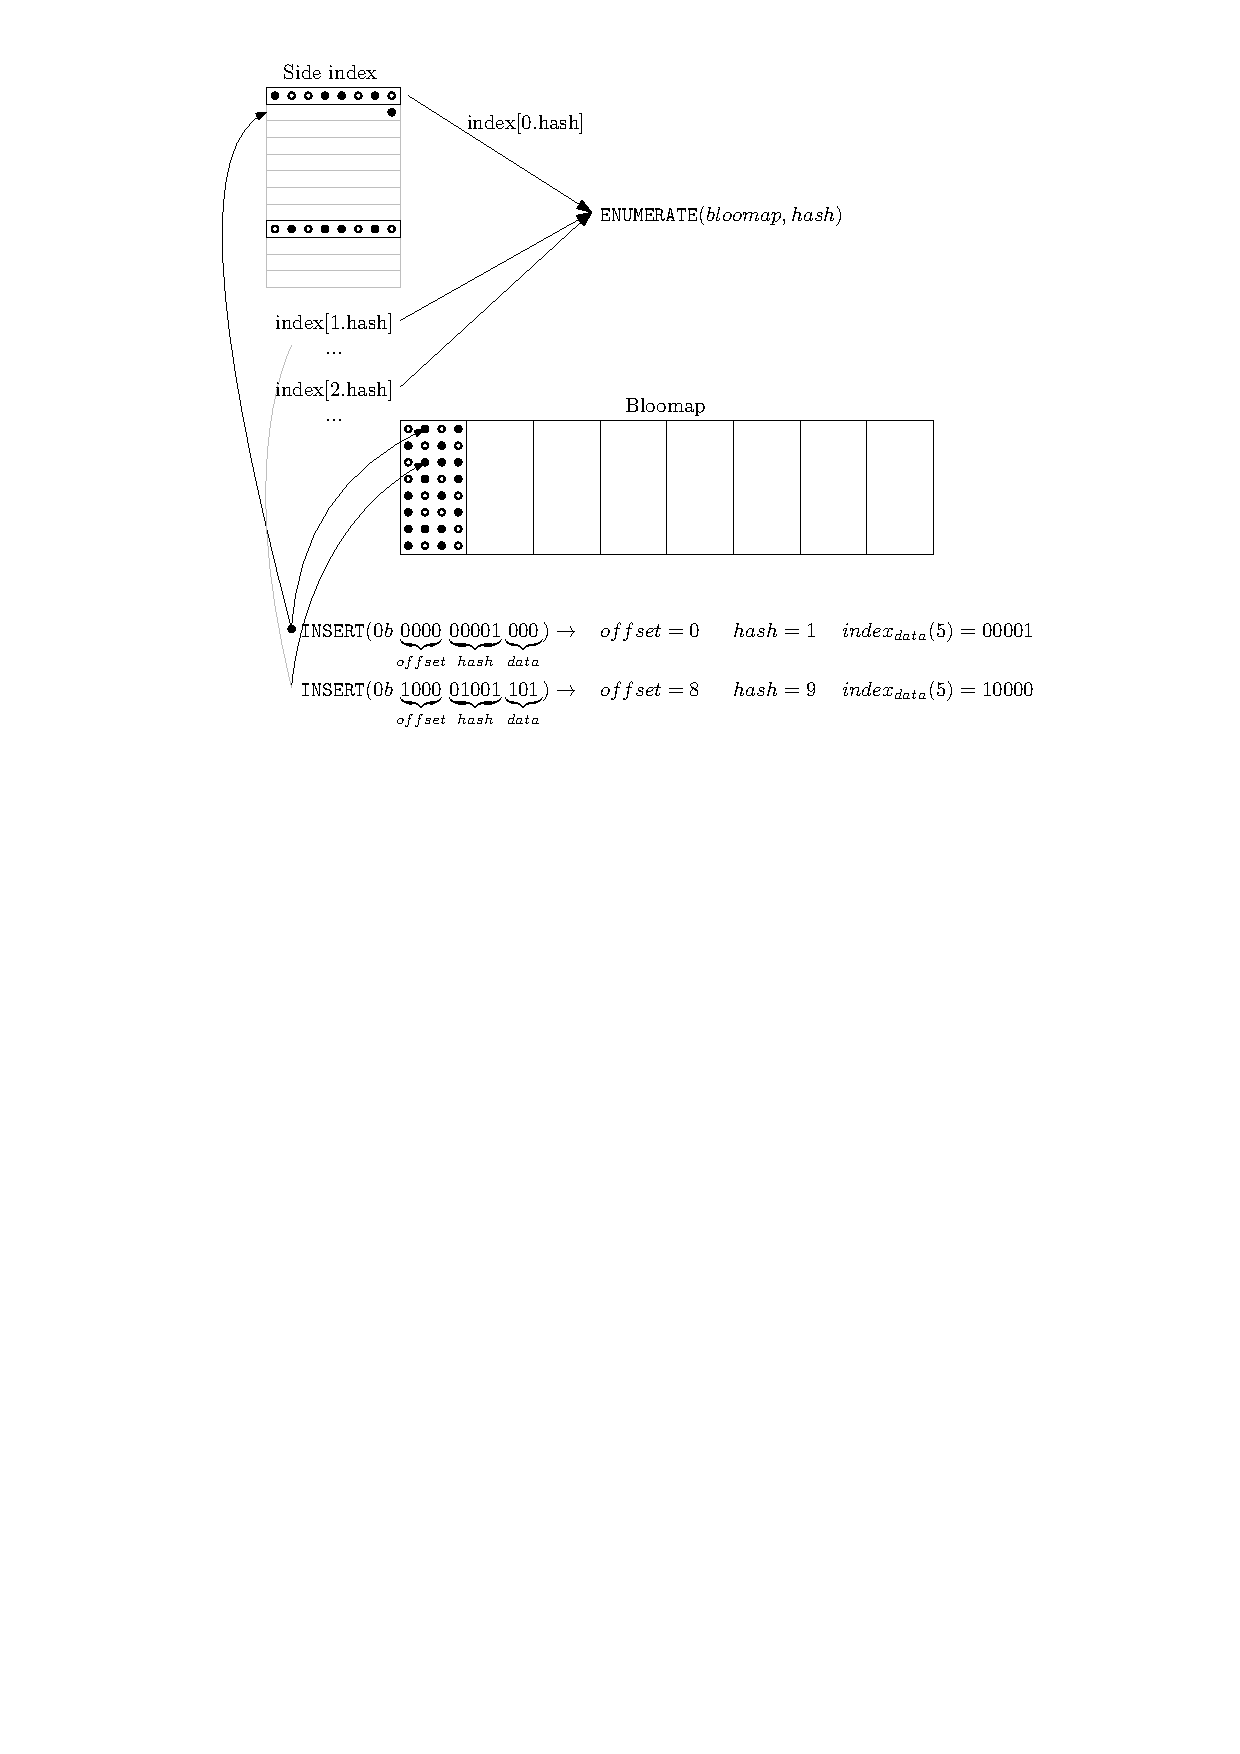
\includegraphics{./img/bloomap_overview.pdf}
	\caption{Overview of Bloomap structure}
	\label{figure-bloomap-overview}
\end{figure}



Both stuctures are pretty straightforward, as {\tt INSERT} is a regular function
for Bloom filter insertion, with the added partition for side index and family
universe insertion.

While insertion in Bloom filter is in $\O(1)$, inserting into a universe may be
$\O(\log n)$ for tree-based implementations or amortized $\O(1)$ for hash-based
implementations. There probably is not a better solution in generic case,
but we suggest a worst-case $\O(1)$ for 32 bit integers (dense sequence of
ids starting from zero).

The Bloomap achieves the following theoretical time complexity:

\begin{itemize}
	\item {\tt QUERY} in $\O(1)$ time.
	\item {\tt INSERT} in $\O(1)$, assuming $\O(1)$ insertion into universe
		index.
	\item {\tt ENUMERATE} in $\O(|U|)$ in worst case, assuming universe index
		suggested in section \ref{sec-compact-representation} and $|U|$ the size
		of the index.
	\item {\tt UNION} in $\O(m)$ time.
	\item {\tt BITWISE\_INTERSECTION} in $\O(m)$ time.
	\item {\tt DELETE{\rm ,} RESIZE} not supported.
\end{itemize}

Though the theoretical complexity of {\tt ENUMERATE} seems very bad, leading
potentially to tens of millions of queries. Here the constant is important, as
the Bloomap will rarely be completely full and most of the queries will be
filtered by the side index and universe index. We can also further optimize the
algorithm to reject enumeration of Bloomap that has more elements than designed
for.

\subsection{Compact representation of dense integer universe}
\label{sec-compact-representation}

Representing universe requires storing sets for different hashes. It is wasteful
to store them in a linked-list, trees or even hash tables, as a humble bit array
fulfills the task. A little unusual form of a bit array has been used, in order
to achieve less allocations and good space efficiency.

As mentioned above, we will split the value to {\tt offset}, {\tt hash} and {\tt
data} at binary boundaries. This means we can simply concatenate the values to
get the represented integer. We can now organize the data into {\it buckets} and
{\it superbuckets} in the following way:

\begin{itemize}
	\item Each {\tt offset} has it's own {\it superbucket}.
	\item Each {\it superbucket} contains a {\it bucket} for every {\tt hash} value.
	\item Each {\it bucket} contains a bit for every {\tt data} value.
\end{itemize}

\begin{center}
	{\tt element = offset$\cdot$hash$\cdot$data} $\Leftrightarrow$
	{\tt universe[offset$\cdot$hash].bit[data]}
\end{center}

\begin{figure}[!ht]
	\centering\hspace{2.5cm}
	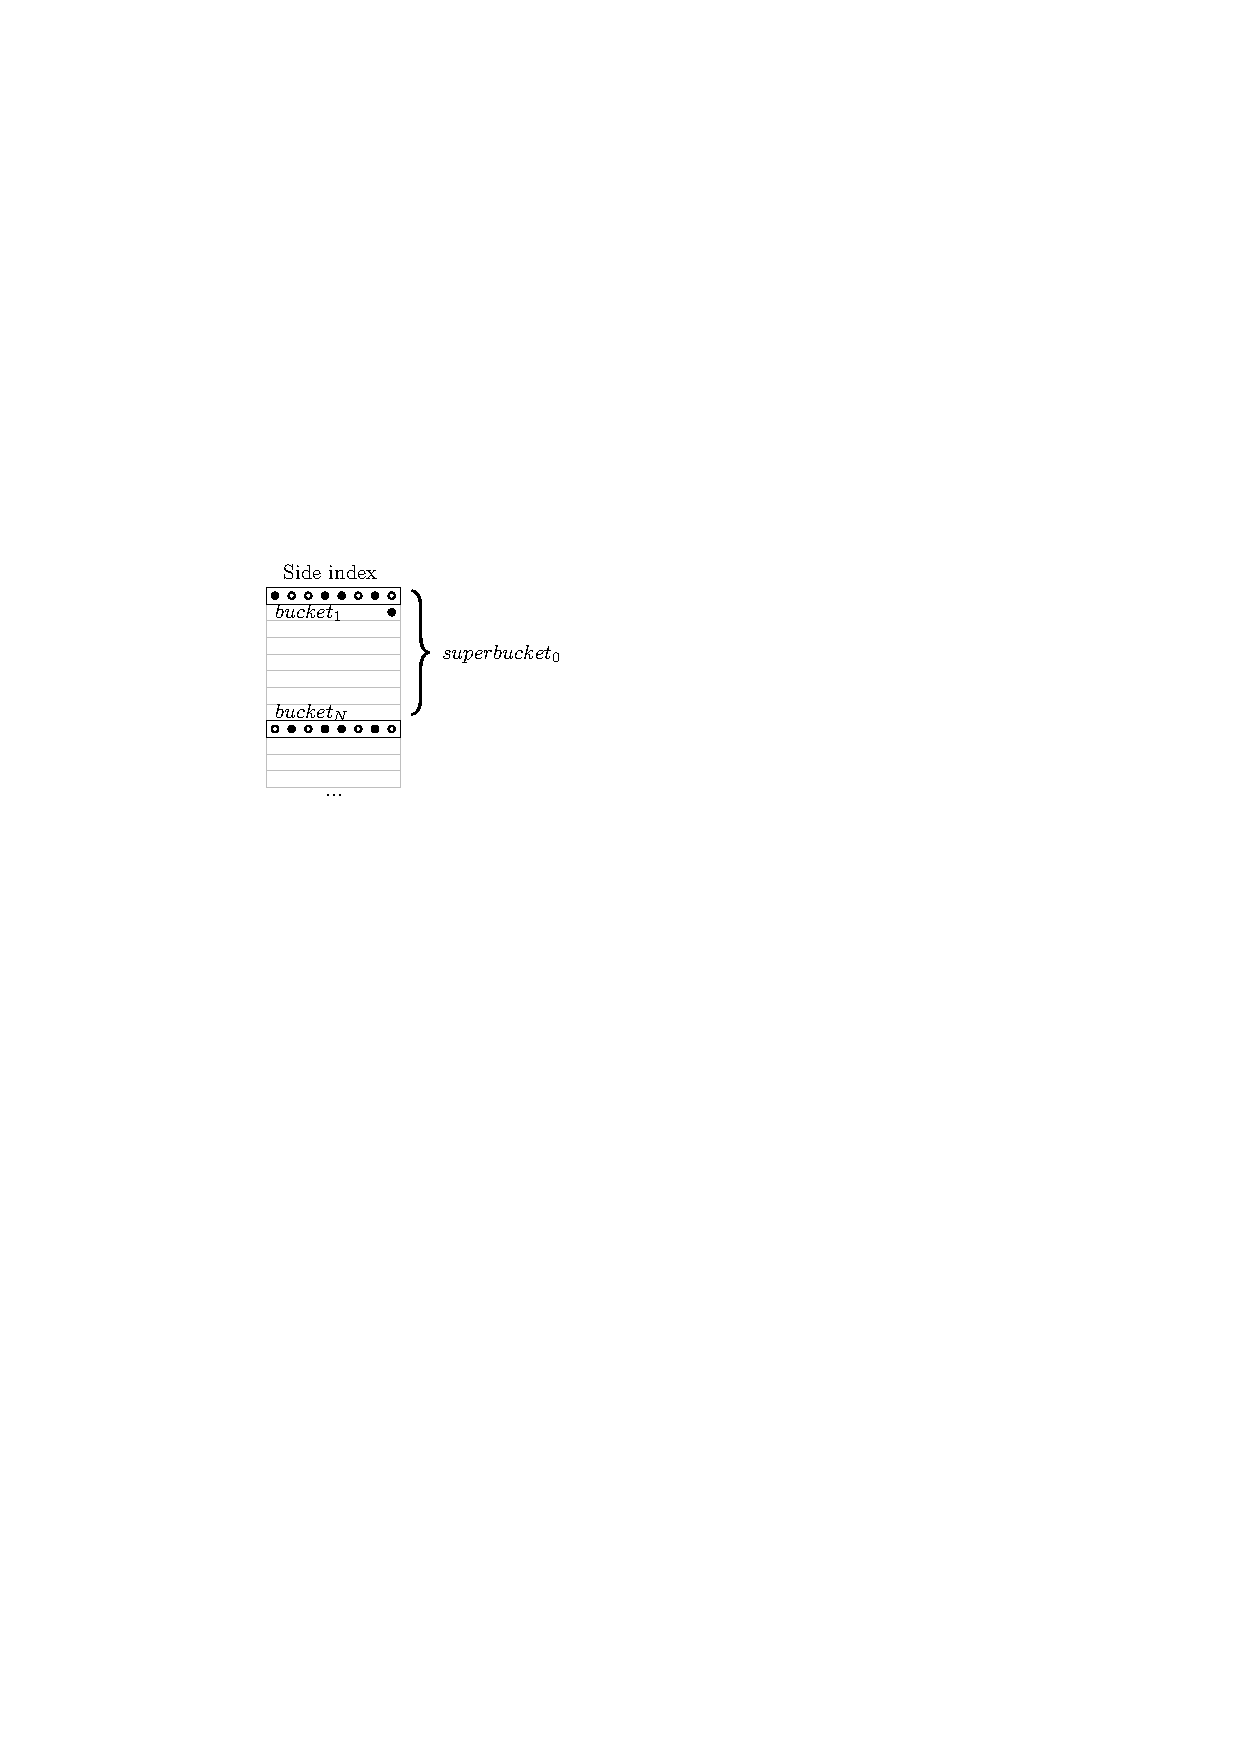
\includegraphics{img/bucketshop.pdf}
	\caption{Bucket and superbuckets in an array.}
	\label{figure-bucketshop}
\end{figure}

The structure is illustrated in Figure \ref{figure-bucketshop} and pseudocode
implementation in Figure \ref{figure-bucketshop-pseudocode}. Memory allocation
is expected to be done automatically in {\tt vector} class and the array should
be resized on first access beyond current boundary.  This allows the structure
to occupy only as much memory as is necessary to store a set of size at most
$\O(\max(E))$, where $E$ is the number of elements inserted. In this case, a
bucket has 64 bits, so it will fit up to 6bit data. Number of bits in hash and
offset is not important and should be chosen by the size of Bloomap's side
index.

\begin{figure}[!ht]
\begin{tcolorbox}
\begin{verbatim}
struct superbucket {
  uint64_t bits[];
};

struct universe_index {
  vector<struct superbucket> superbuckets;
};

void universe_index::INSERT(offset, hash, data) {
  superbuckets[offset]->bits[hash].bit[data] = 1;
}

vector<element> universe_index::ENUMERATE(hash) {
  vector<element> candidates;
  for (sb in superbuckets) {
    for (i = 0 .. 63) {
      if (sb->bits[hash].bit[i]) 
        candidates.append(bit);
    }
  }
  return candidates;
}
\end{verbatim}
\end{tcolorbox}
\caption{Bucket and superbuckets prototype and pseudocode}
	\label{figure-bucketshop-pseudocode}
\end{figure}

\begin{figure}[!ht]
\begin{tcolorbox}
\begin{verbatim}
struct Bloomap {
  BloomapFamily f;            # Family this maps belongs to
  int m,k,s;                  # Filter parameters

  int index[s];               # Side index
  int partitions[k][m/k];     # Regular filter partitions
};

struct BloomapFamily {
  vector Bloomap;             # Owned bloomaps
  int m,k,s;                  # Filter parameters

  hash_set universe;          # Indexed universe
}
\end{verbatim}
\end{tcolorbox}
	\caption{Bloomap and BloomapFamily prototypes (in pseudocode)}
\label{figure-bloomap-decl}
\end{figure}

\begin{figure}[!ht]
\begin{tcolorbox}
\begin{verbatim}
void Bloomap::INSERT(element) {
  # Decompose element to offset, index_hash and data.
  (offset,index_hash,data) := element;
  # Insert into side index of a bloomap.
  index[index_hash] := true;
  for (i := 1..k) {
    partitions[i][hash_fn(i,element) % m/k] := 1
  }
  # Insert into universe index of a family
  f.universe[index_hash] += element;
}

bool Bloomap::QUERY(element) {
  for (i := 1..k) {
    if (partitions[i][hash_fn(i,element) % m/k] == 0)
      return false;
  }
  return true;
}

void Bloomap::UNION(another) {
  for (i := 1..s) {
    index[i] |= another.index[i];
  }
  for (i := 1..k, j := 0..m/k) {
    partitions[i][j] |= another.partitions[i][j];
  }
}

vector Bloomap::ENUMERATE() {
  vector list = ();
  # Check each element in side index
  for (i := 1..s | index[i] == true) {
    # Test for every element universe lists for this index
    for (element in f.universe[i] && this.QUERY(element)) 
      list += element;
  }
  return list;
}

\end{verbatim}
\end{tcolorbox}
\caption{Basic Bloomap operations (in pseudocode)}
\label{figure-bloomap-fn}
\end{figure}

\chapter{Misc stuff -- to be moved elsewhere}
\section{Experimenting with GCC}

As I previously noted, I will be focusing on the GCC compiler suite. In this
section, I will cover the experimental setup, compile a few programs and extract
some practical information on resources needed and anticipated use.

The raw data gained in this chapter will not be published, as they tend to be
rather large. I will however publish source code used to take these
measurements, so anyone can reproduce these results, and perhaps use for
comparison on his/her own work. I will also omit some technical details in this
chapter, but will include them in the Appendix \TODO{link}.

\subsection{The setup}

\subsection{Compiler}

For further measurements, I will be using GCC compiled from branch {\tt
gcc-5-branch} (via github.com mirror, but any up to date repository will
suffice). The reason for this branch is simple: it's relatively fresh branch,
that supports most of the latest features, but will not change during
development and provide stable base for testing, while still receiving bug fixes
for the time being.

This is especially important due to the fact that some newer releases have
trouble compiling software like Firefox, which is essentil for some of my
benchmarks. I could fix those, it isn't worth the trouble to do so, and the best
performing code will be ported to the current master branch.

Also, the GCC is non-bootstrapped, but compiled with a system-installed compiler
of the same version, so there should be little to no performance hit. However,
what comes with a performance hit are the benchmarking outputs themselves,
though I will note the time spent in the benchmarking code if it's significant.

\subsection{Software under test}

I have checked many opensource programs to pick some candidates, that could
serve as test inputs. I had a few requirements, to make testing straightforward
and reproducible:

\begin{itemize}
	\item Written in C++ (preferred) or C.
	\item A good compatibility with current GCC versions (5.x and 6.x)
	\item Flexible and robust build system.
	\item Mid to large codebase.
	\item Not too modular.
\end{itemize}

It's suprisingly difficult to find projects that fit all of those, but all of
them are very important. Among others, I first considered well-known projects
like Firefox, GIMP, Inkscape, MySQL and SQLite. I ruled out Inkscape and MySQL


\chapter*{Conclusion}
\addcontentsline{toc}{chapter}{Conclusion}


\appendix
\chapter{GCC cookbook}

Working on GCC is not easy, as it's not a program like others. It's a suite of
compilers\footnote{GCC stands for GNU Compiler Collection}, but contains some
other libraries (for example, the C++ standard library). Moreover, to test our
results, we need to invoke the newly compiled compiler, instead of the system
one. This appendix contains some useful tips, that should be enough to test all
the provided code and replicate the results.

\section{Compiling GCC}

As any other package utilizing {\tt autotools}, GCC can be compiled by a simple
{\tt ./configure \&\& make \&\& make install}. Besides the usual needs, as
configuring a proper prefix (so it won't overwrite our system files), this
approach has several other limitations. For the most part, it takes way too
long to build, as it builds all the language frontends and bootstraps itself.
The process of bootstrapping serves two main function, to test the new compiler
and to provide a more optimized version (for example, if the compiler on host
system was too old to support some optimizations).

Both of these features are good and useful in most cases. None of them is
useful in development and debugging. Let's see why:

\paragraph{Bootstrap.} It compiles GCC three times in a row, each time with the
previous version. This not only takes time, but makes debugging harder, as we
now have the additional need to identify, if a given manifestation is a direct
result of our bug, or a result of miscompiled first (or later) stage.

\paragraph{Language frontends.} GCC itself is written mostly in C/C++, and
those are the only languages required to build a working compiler. Building
frontends that won't be tested is a waste of time.

\paragraph{Multilib.} Provides support for running 32bit code on 64bit
machines. We usually won't need it for development.

After taking all of this into account, let's see how our build will look:

\begin{verbatim}
mkdir obj-build; cd obj-build
../configure --prefix=$HOME/gcc/dev --enable-languages=c++,c \
   --disable-bootstrap --enable-maintainer-mode --disable-multilib
make
make install
\end{verbatim}

A build out of repository root is recommended (we used obj-build), maintainer
is required if configuration for autotools or automake was changed (it was in
this project).

After this, we have a working compiler ready to use, in {\tt \$HOME/gcc/dev}.
This path can be inserted into the PATH system variable, to prefer our new
development compiler.

One of the attachments is a handy script that handles all of this, and provides
not only easy to use interface, but also reproducibility of results.

\section{Runtime libraries}

As mentioned above, the runtime library is part of the GCC suite. It's usually
built during the first build, and never touch again unless it's sources were
changed. This gives us an opportunity to cheat little: building the runtime
with a known working compiler, and commit the changes under scrutiny after the
runtime is built. This gives us the assurance that bugs we are seeing are
directly caused by our compiler, not by a miscompilation of runtime library.

One of the usual symptoms follows: after a unsuccessful modification the
changes are reset and a known working version is checked-out, the new compiler
may seem to be still malfunctioning. This may be caused by a miscompiled
runtime, built with the (buggy) experimental compiler.


%%% Bibliography
%%% Bibliography (literature used as a source)
%%%
%%% We employ bibTeX to construct the bibliography. It processes
%%% citations in the text (e.g., the \cite{...} macro) and looks up
%%% relevant entries in the bibliography.bib file.
%%%
%%% The \bibliographystyle command selects, which style will be used
%%% for references from the text. The argument in curly brackets is
%%% the name of the corresponding style file (*.bst). Both styles
%%% mentioned in this template are included in LaTeX distributions.

\bibliographystyle{plainnat}    %% Author (year)
% \bibliographystyle{unsrt}     %% [number]

\renewcommand{\bibname}{Bibliography}

%%% Generate the bibliography. Beware that if you cited no works,
%%% the empty list will be omitted completely.

\nocite{*}
\bibliography{bibliography}

%%% If case you prefer to write the bibliography manually (without bibTeX),
%%% you can use the following. Please follow the ISO 690 standard and
%%% citation conventions of your field of research.

% \begin{thebibliography}{99}
%
% \bibitem{lamport94}
%   {\sc Lamport,} Leslie.
%   \emph{\LaTeX: A Document Preparation System}.
%   2nd edition.
%   Massachusetts: Addison Wesley, 1994.
%   ISBN 0-201-52983-1.
%
% \end{thebibliography}



[Guo10]
D. Guo, J. Wu, H. Chen, Y. Yuan, and X. Luo. The
dynamic Bloom filters.
IEEE Transactions on
Knowledge and Data Engineering
, 22:120–133, 2010.q


%%% Figures used in the thesis (consider if this is needed)
\listoffigures

%%% Tables used in the thesis (consider if this is needed)
%%% In mathematical theses, it could be better to move the list of tables to the beginning of the thesis.
\listoftables

%%% Abbreviations used in the thesis, if any, including their explanation
%%% In mathematical theses, it could be better to move the list of abbreviations to the beginning of the thesis.
\chapwithtoc{List of Abbreviations}

%%% Attachments to the master thesis, if any. Each attachment must be
%%% referred to at least once from the text of the thesis. Attachments
%%% are numbered.
%%%
%%% The printed version should preferably contain attachments, which can be
%%% read (additional tables and charts, supplementary text, examples of
%%% program output, etc.). The electronic version is more suited for attachments
%%% which will likely be used in an electronic form rather than read (program
%%% source code, data files, interactive charts, etc.). Electronic attachments
%%% should be uploaded to SIS and optionally also included in the thesis on a~CD/DVD.
\chapwithtoc{Attachments}

\openright
\end{document}
